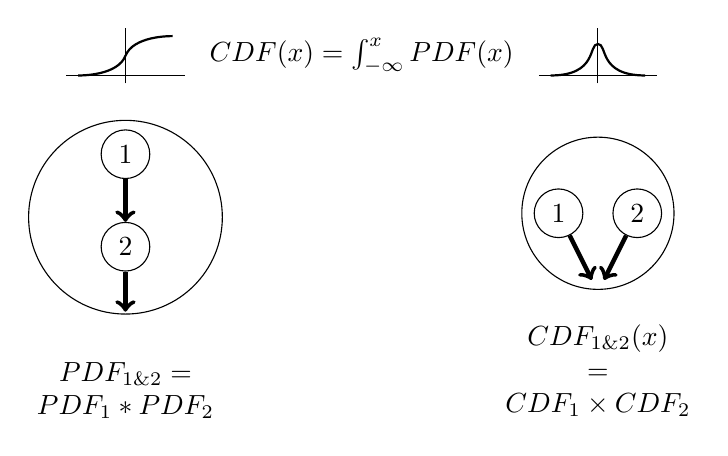
\begin{tikzpicture}[
task/.style={draw,circle},
arw/.style={->,ultra thick}
]
%\draw[help lines](-5,-3)grid(5,3);
\begin{scope}[shift={(0,2.5)}]
\node[]at(0,0){$CDF(x)=\int_{-\infty}^xPDF(x)$};
\begin{scope}[scale=0.5,shift={(-6,-0.5)}]
\draw(-1.5,0)--(1.5,0);
\draw(0,-0.2)--(0,1.2);
\draw[thick](-1.2,0) ..controls (-1.1,0) and (-0.2,0)  .. (0,0.5) .. controls (0.2,1) and (1.1,1) .. (1.2,1);
\end{scope}
\begin{scope}[scale=0.5,shift={(6,-0.5)}]
\draw(-1.5,0)--(1.5,0);
\draw(0,-0.2)--(0,1.2);
\draw[thick](-1.2,0) ..controls (0,0) and (-0.25,0.8) .. (0,0.8) ..controls (0.25,0.8) and (0,0) .. (1.2,0);
\end{scope}
\end{scope}

\begin{scope}[shift={(-3,-0.75)}]
\node[task]at(0,2)(1){1};
\node[task]at(0,0.825)(2){2};
\node[task,minimum width=70]at(0,1.2){};
\draw[arw](1)--(2);
\draw[arw](2)--(0,0); 
\node[align=center]at(0,-1){$PDF_{1\&2}=$\\$PDF_1* PDF_2$};
\end{scope}

\begin{scope}[shift={(3,0-0.5)}]
\node[circle]at(0,0)(0){};
\node[task]at(-0.5,1)(1){1};
\node[task]at(0.5,1)(2){2};
\node[task,minimum width=55]at(0,1){};
\draw[arw](1)--(0);
\draw[arw](2)--(0); 
\node[align=center]at(0,-1){$CDF_{1\&2}(x)$\\$=$\\$CDF_1\times{}CDF_2$};
\end{scope}

\end{tikzpicture}
